\documentclass[border=3mm]{standalone}\usepackage[]{graphicx}\usepackage[]{color}
%% maxwidth is the original width if it is less than linewidth
%% otherwise use linewidth (to make sure the graphics do not exceed the margin)
\makeatletter
\def\maxwidth{ %
  \ifdim\Gin@nat@width>\linewidth
    \linewidth
  \else
    \Gin@nat@width
  \fi
}
\makeatother

\definecolor{fgcolor}{rgb}{0.345, 0.345, 0.345}
\newcommand{\hlnum}[1]{\textcolor[rgb]{0.686,0.059,0.569}{#1}}%
\newcommand{\hlstr}[1]{\textcolor[rgb]{0.192,0.494,0.8}{#1}}%
\newcommand{\hlcom}[1]{\textcolor[rgb]{0.678,0.584,0.686}{\textit{#1}}}%
\newcommand{\hlopt}[1]{\textcolor[rgb]{0,0,0}{#1}}%
\newcommand{\hlstd}[1]{\textcolor[rgb]{0.345,0.345,0.345}{#1}}%
\newcommand{\hlkwa}[1]{\textcolor[rgb]{0.161,0.373,0.58}{\textbf{#1}}}%
\newcommand{\hlkwb}[1]{\textcolor[rgb]{0.69,0.353,0.396}{#1}}%
\newcommand{\hlkwc}[1]{\textcolor[rgb]{0.333,0.667,0.333}{#1}}%
\newcommand{\hlkwd}[1]{\textcolor[rgb]{0.737,0.353,0.396}{\textbf{#1}}}%

\usepackage{framed}
\makeatletter
\newenvironment{kframe}{%
 \def\at@end@of@kframe{}%
 \ifinner\ifhmode%
  \def\at@end@of@kframe{\end{minipage}}%
  \begin{minipage}{\columnwidth}%
 \fi\fi%
 \def\FrameCommand##1{\hskip\@totalleftmargin \hskip-\fboxsep
 \colorbox{shadecolor}{##1}\hskip-\fboxsep
     % There is no \\@totalrightmargin, so:
     \hskip-\linewidth \hskip-\@totalleftmargin \hskip\columnwidth}%
 \MakeFramed {\advance\hsize-\width
   \@totalleftmargin\z@ \linewidth\hsize
   \@setminipage}}%
 {\par\unskip\endMakeFramed%
 \at@end@of@kframe}
\makeatother

\definecolor{shadecolor}{rgb}{.97, .97, .97}
\definecolor{messagecolor}{rgb}{0, 0, 0}
\definecolor{warningcolor}{rgb}{1, 0, 1}
\definecolor{errorcolor}{rgb}{1, 0, 0}
\newenvironment{knitrout}{}{} % an empty environment to be redefined in TeX

\usepackage{alltt}
\usepackage{tikz}
\usetikzlibrary{arrows,positioning}
\IfFileExists{upquote.sty}{\usepackage{upquote}}{}
\begin{document}





%%%%%%%%%%%%%%%%%%%%%%%%%%%%%%%%%%%%%%%%%%%%%%%%%%%%%%%%%%%%%%%%%%%%%%%%%%%%%%%%%%%%%
% MLSEM_fin
%%%%%%%%%%%%%%%%%%%%%%%%%%%%%%%%%%%%%%%%%%%%%%%%%%%%%%%%%%%%%%%%%%%%%%%%%%%%%%%%%%%%%

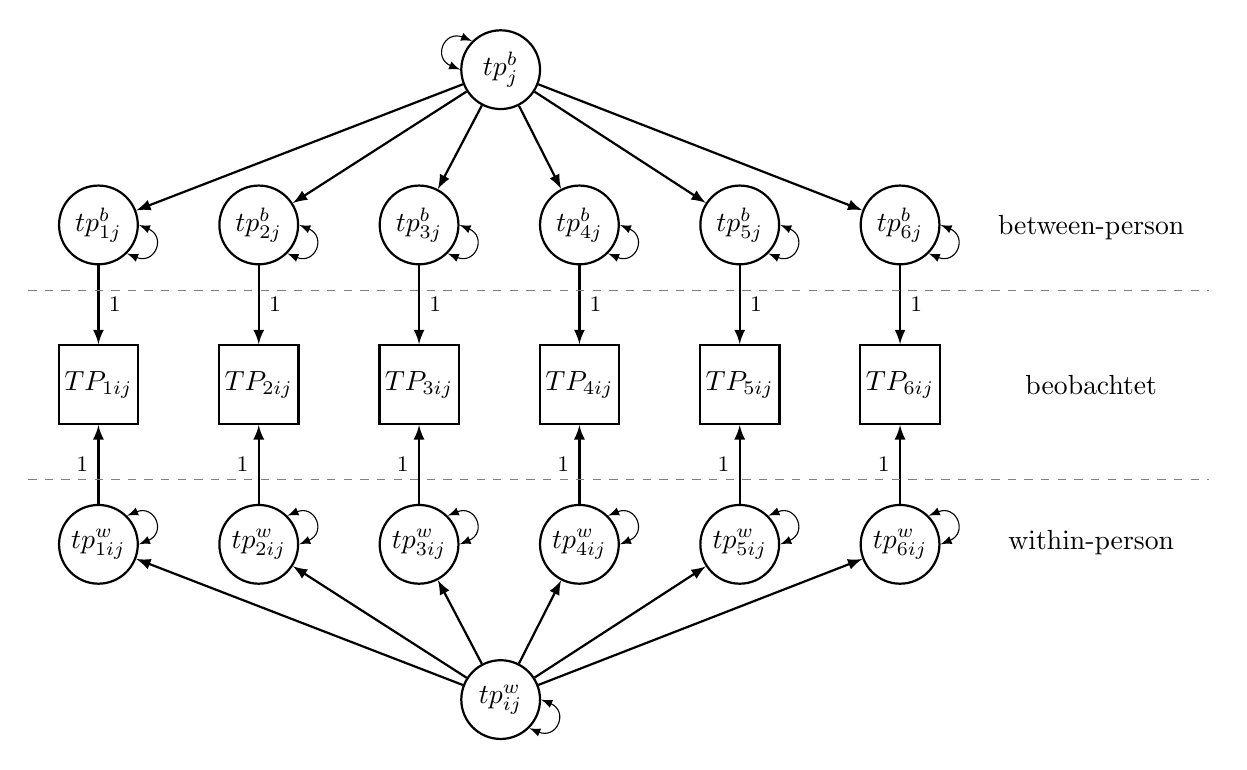
\begin{tikzpicture}[auto,>=latex,align=center,
latent/.style={circle,draw, thick,inner sep=0pt,minimum size=10mm},
manifest/.style={rectangle,draw, thick,inner sep=2pt,minimum size=10mm},
manifestcov/.style={rectangle,draw, thick,inner sep=1pt,minimum size=8mm},
mean/.style={regular polygon,regular polygon sides=3,draw,thick,inner sep=0pt,minimum size=10mm},
paths/.style={->, thick, >=latex, font = \footnotesize, fill = white},
variance/.style={<->, thin, >=latex, bend left=270, looseness=2.5, font = \footnotesize},
dotsdots/.style={circle, draw, fill = black, minimum size = 2mm}
]

%% Nodes   %%%%%%%%%%%%%%%%%%%%%%%%%%%%%%%%%%%%%%%%%%%%%%%%%%%%%%%%%%%%%%%%%%%%%%%

%% Latente Variablen
\node [latent] (TPB) at (0,2)  {$tp^{b}_{j}$};
\node [latent] (TPW) at (0,-6)  {$tp^{w}_{ij}$};


%% Manifeste Items
\node [manifest] (TP4) at (+1,-2)       {$TP_{4ij}$};
\node [manifest] (TP3) [left  =of TP4]  {$TP_{3ij}$};
\node [manifest] (TP2) [left  =of TP3]  {$TP_{2ij}$};
\node [manifest] (TP1) [left  =of TP2]  {$TP_{1ij}$};
\node [manifest] (TP5) [right =of TP4]  {$TP_{5ij}$};
\node [manifest] (TP6) [right =of TP5]  {$TP_{6ij}$};

%% Random Intercept
\node [latent] (EB1) [above =of TP1]  {$tp^{b}_{1j}$};    
\node [latent] (EB2) [above =of TP2]  {$tp^{b}_{2j}$};    
\node [latent] (EB3) [above =of TP3]  {$tp^{b}_{3j}$}; 
\node [latent] (EB4) [above =of TP4]  {$tp^{b}_{4j}$};  
\node [latent] (EB5) [above =of TP5]  {$tp^{b}_{5j}$}; 
\node [latent] (EB6) [above =of TP6]  {$tp^{b}_{6j}$};   

%% Level 1 Errors
\node [latent] (EW1) [below =of TP1]  {$tp^{w}_{1ij}$};
\node [latent] (EW2) [below =of TP2]  {$tp^{w}_{2ij}$};
\node [latent] (EW3) [below =of TP3]  {$tp^{w}_{3ij}$};
\node [latent] (EW4) [below =of TP4]  {$tp^{w}_{4ij}$};
\node [latent] (EW5) [below =of TP5]  {$tp^{w}_{5ij}$};
\node [latent] (EW6) [below =of TP6]  {$tp^{w}_{6ij}$};



%% Pfade %%%%%%%%%%%%%%%%%%%%%%%%%%%%%%%%%%%%%%%%%%%%%%%%%%%%%%%%%%%%%%%%%%%%%%%%%%%

%% Pfade Messmodelle Between
\draw [paths] (TPB) to node {} (EB1);
\draw [paths] (TPB) to node {} (EB2);
\draw [paths] (TPB) to node {} (EB3);
\draw [paths] (TPB) to node {} (EB4);
\draw [paths] (TPB) to node {} (EB5);
\draw [paths] (TPB) to node {} (EB6);

\draw [paths] (EB1) to node {1} (TP1);
\draw [paths] (EB2) to node {1} (TP2);
\draw [paths] (EB3) to node {1} (TP3);
\draw [paths] (EB4) to node {1} (TP4);
\draw [paths] (EB5) to node {1} (TP5);
\draw [paths] (EB6) to node {1} (TP6);

%% Pfade Messmodelle Within
\draw [paths] (TPW) to node {} (EW1);
\draw [paths] (TPW) to node {} (EW2);
\draw [paths] (TPW) to node {} (EW3);
\draw [paths] (TPW) to node {} (EW4);
\draw [paths] (TPW) to node {} (EW5);
\draw [paths] (TPW) to node {} (EW6);

\draw [paths] (EW1) to node {1} (TP1);
\draw [paths] (EW2) to node {1} (TP2);
\draw [paths] (EW3) to node {1} (TP3);
\draw [paths] (EW4) to node {1} (TP4);
\draw [paths] (EW5) to node {1} (TP5);
\draw [paths] (EW6) to node {1} (TP6);




%% Pfade Varianzen
\foreach \x/\xlab in {EW1/, EW2/,EW3/, EW4/, EW5/, EW6/}
\draw [variance, above] (\x.east) to node [swap] {\xlab}  (\x.north east);

\foreach \x/\xlab in {EB1/, EB2/, EB3/, EB4/, EB5/, EB6/}
\draw [variance] (\x.south east) to node [swap] {\xlab}  (\x.east);

\foreach \x/\xlab in {TPB/}
\draw [variance] (\x.north west) to node [swap] {\xlab}  (\x.west);

\foreach \x/\xlab in {TPW/}
\draw [variance] (\x.south east) to node [swap] {\xlab}  (\x.east);






%% Level-Lines & Text %%%%%%%%%%%%%%%%%%%%%%%%%%%%%%%%%%%%%%%%%%%%%%%%%%%%%%%%%%%%%%%
\draw[gray, dashed] (-6,-0.8) -- (9,-0.8);
\draw[gray, dashed] (-6,-3.2) -- (9,-3.2);

\node[draw = white,text width=3cm] at (7.5,-2) {beobachtet};
\node[draw = white,text width=3cm] at (7.5, 0) {between-person};
\node[draw = white,text width=3cm] at (7.5,-4) {within-person};

\end{tikzpicture}

\end{document}
